\chapter{Metriche}

In questo capitolo verranno descritte le metriche anticipate nella Sezione
\ref{descrizione_progetto}, mostrando il relativo codice e i risultati ottenuti.

\section{Metriche sulle conferenze}

Questa sezione tratta delle varie metriche relative all'insieme di conferenze
analizzate, che conta un totale di più di 500 conferenze.

\subsection{Rating delle conferenze}

Come descritto in Sezione~\ref{sec:conferenze}, le conferenze possono avere
un rating, rappresentato da una lettera, che rappresenta la qualità generale
della conferenza.

Al fine di comprendere al meglio come questa classifica influenza i vari indici
bibliometrici, in Figura~\ref{fig:conferences-distribution} viene rappresentata
la suddivisione delle conferenze in base alla loro qualità come classificata
dal GGS.

\begin{figure}[tb]
  \centering
  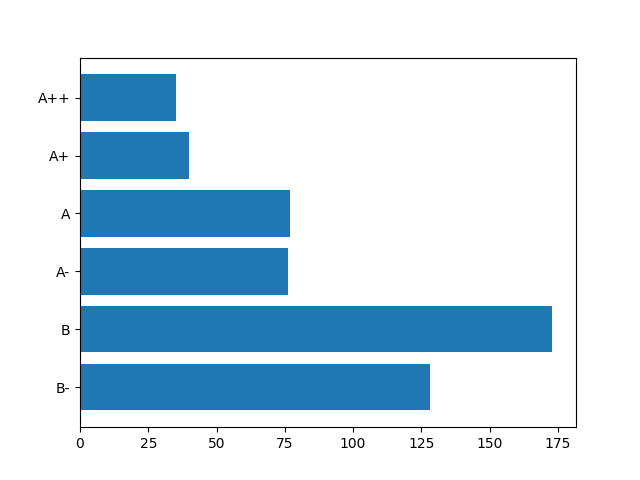
\includegraphics[width=\linewidth]{conferences-distribution.png}
  \caption{Distribuzione delle conferenze}
  \label{fig:conferences-distribution}
\end{figure}

È immediato notare che la distribuzione è suddivisa in 3 gruppi principali:
\begin{enumerate}
  \item Il gruppo delle ``conferenze top'', dato dalle A++ e dalle A+, che
        risulta essere il più contenuto di tutti con meno di 100 conferenze;
  \item Il secondo gruppo delle conferenze di alto livello, dato dalle A e A-,
        che risulta comunque non molto più grande del precedente con circa 150
        conferenze;
  \item Ed infine il gruppo delle conferenze B e B-, che domina in quanto a numero
        i precedenti due, avendo più conferenze degli altri due gruppi combinati.
\end{enumerate}

Questo conferma quello che ci si può aspettare in generale con la classificazione
generale per qualità in molti ambiti: in generale, la qualità alta è correlata
con una numerosità minore.

Ciò fa sì che conferenze con qualità più alta, essendo in numero minore,
ricevano una competizione maggiore rispetto a quelle di qualità più bassa, in
quanto una conferenza di ottimo livello tenderà ad essere più critica sui lavori
ricevuti al fine di mantenere tale ranking. D'altra parte, una conferenza con
ranking minore potrebbe puntare maggiormente sulla quantità di paper al fine di
crescere di dimensioni per poter avere una possibilità di salire di ranking,
ma a scapito del controllo della qualità dei lavori ad essa sottomessi.

\subsection{Numero di citazioni per paper in base al rating}

Si vuole ora guardare a come la qualità di una conferenza influenza il numero
di citazioni che un paper prende in media. Il numero di citazioni di un paper
è una metrica importante per un ricercatore, in quanto è uno dei fattori
che contribuisce ai suoi indici principali, tra cui l'$h$-index.

La Figura~\ref{fig:paper-rating-distribution} mostra appunto tale distribuzione,
rappresentando con un punto il numero di citazioni di ogni singolo paper e
con una linea rossa la media di citazioni in base al rating della conferenza
a cui il paper è stato sottomesso. I valori di tale media sono visibili
anche in Tabella~\ref{table:paper-rating-distribution}.

\begin{figure}[tb]
  \centering
  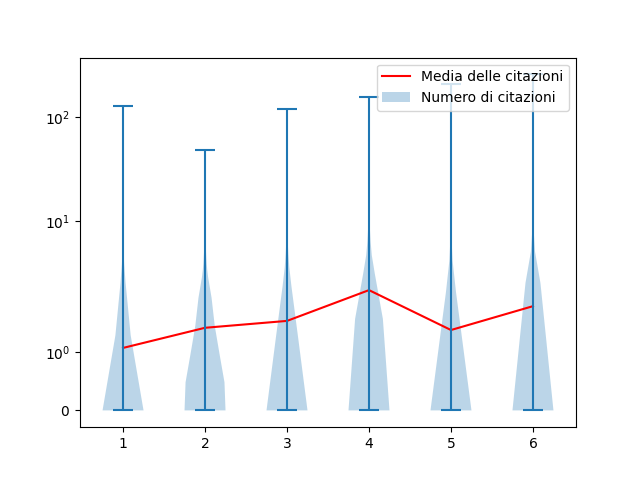
\includegraphics[width=\linewidth]{paper_rating_distribution.png}
  \caption{Numero di citazioni per conferenza}
  \label{fig:paper-rating-distribution}
\end{figure}

\begin{table}[tb]
  \centering
  \begin{tabular}{||l | r ||}
    \hline
    \textbf{Rating conferenza} & \textbf{Numero di citazioni medio} \\ [0.5ex] 
    \hline\hline
    A++    & 1.075884 \\ \hline
    A+     & 1.422904 \\ \hline
    A      & 1.541459 \\ \hline
    A-     & 2.191858 \\ \hline
    B      & 1.384308 \\ \hline
    B-     & 1.795274 \\ \hline
  \end{tabular}
  \caption{Numero di citazioni medio per rating}
  \label{table:paper-rating-distribution}
\end{table}

Dall'immagine è possibile trarre due conclusioni importanti:
\begin{enumerate}
  \item La prima è che, in media, le citazioni per un paper sono basse sul
        periodo di qualche anno che è stato considerato;
  \item La seconda, invece, è che la distribuzione delle citazioni è molto sbilanciata,
        in quanto ci sono molti paper con poche citazioni e pochi paper che superano
        le 150 citazioni.
\end{enumerate}

Queste due conclusioni valgono inoltre per qualsiasi ranking di conferenza,
con un leggero aumento per le conferenze di livello inferiore.
Si può quindi dedurre che, in genere, il livello di una conferenza non influenza
il numero di citazioni ottenute nel breve periodo ($\sim$5 anni), con anzi
un aumento delle citazioni in media per conferenze non top, ovvero con ranking
da A in giù.

\subsection{Media dell'$h$-index per conferenza in base al rating}

Oltre al numero di citazioni, è interessante guardare anche
a come l'$h$-index degli autori è correlato con il rating delle conferenze
a cui partecipano. Questo perché ci si aspetta che conferenze con un rating
maggiore attirino ricercatori con più esperienza, in quanto il loro
processo di accettazione è sicuramente più selettivo rispetto a conferenze
più nuove oppure semplicemente classificate come di livello inferiore.

Nella Figura~\ref{fig:h-index-vs-rating} si vede appunto questa metrica,
rappresentata tramite un grafico a violino con in rosso la media dell'$h$-index
per rating della conferenza, i cui valori precisi sono visibili in
Tabella~\ref{table:h-index-vs-rating}.

\begin{figure}[tb]
  \centering
  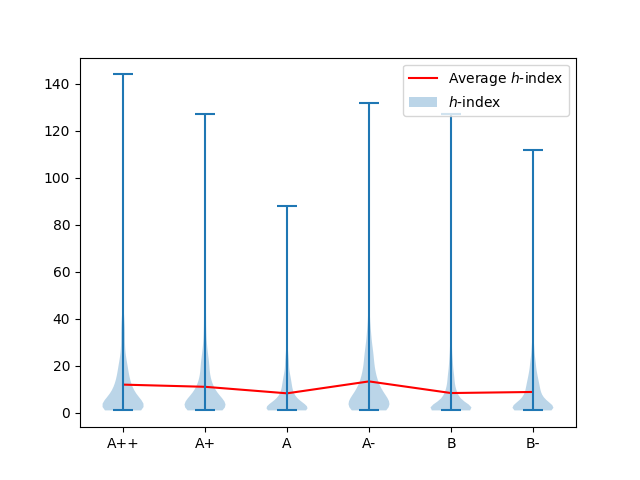
\includegraphics[width=\linewidth]{h_index_vs_conference_rating.png}
  \caption{$h$-index per conferenza}
  \label{fig:h-index-vs-rating}
\end{figure}

\begin{table}[tb]
  \centering
  \begin{tabular}{||l|r||}
    \hline
    \textbf{Rating conferenza} & \textbf{$h$-index medio} \\ [0.5ex] 
    \hline\hline
    A++    & 11.97 \\ \hline
    A+     & 11.04 \\ \hline
    A      & 8.27  \\ \hline
    A-     & 13.34 \\ \hline
    B      & 8.39 \\ \hline
    B-     & 8.84 \\ \hline
  \end{tabular}
  \caption{Valori medi dell'$h$-index}
  \label{table:h-index-vs-rating}
\end{table}

Come si può vedere dai dati, per le conferenze di livello ottimo (A++ e A+)
si ha un $h$-index maggiore in media, pari a circa $11.51$, rispetto a quelle
degli altri due livelli ($10.81$ per le conferenze A e A-, $8.62$ per le B e
B-).

Questo coincide con le aspettative: conferenze di livello maggiore hanno
un processo selettivo più restrittivo e di conseguenza è più probabile
che un ricercatore con più esperienza (e quindi con $h$-index probabilmente
più alto) sottoponga lavori a queste conferenze.

Notare comunque che la differenza fra le varie categorie non è così elevata,
e le curve sono fortemente sbilanciate verso $h$-index bassi in ogni caso,
anche se ciò è più visibile nelle conferenze di rating B e B-.

% \chapter{Metriche}
%In questo capitolo verranno descritte le metriche anticipate nella Sezione \ref{descrizione_progetto}, mostrando il relativo codice e i risultati ottenuti.

%\section{Distribuzione della qualità delle conferenze}


%\section{Distribuzione degli H-index degli autori}
%\section{Distribuzione della qualità dei lavori per autore}
%\section{Correlazione tra qualità delle conferenze e numero di citazioni del paper}
%\section{Correlazione tra qualità della conferenza e distribuzione degli H-index degli autori coinvolti}